\documentclass[a4paper,12pt]{article}
\usepackage[margin=18mm]{geometry}
\usepackage{tikz}
\usepackage{amsmath}
\usepackage{xcolor}
\newcommand{\pFourCell}[2]{\makebox[#1em][c]{\ensuremath{#2}}}
\newcommand{\pFourCenterBox}[1]{\begingroup\setbox0=\hbox{$\displaystyle #1$}\dimen0=\ht0\advance\dimen0 by -\dp0\divide\dimen0 by 2\lower\dimen0\box0\endgroup}
\newdimen\pFourFractionRuleThickness
\pFourFractionRuleThickness=0.4pt
\newcommand{\pFourTopAlign}[3]{\raisebox{-#1}[0pt][\dimexpr #1 + #2\relax]{\ensuremath{\displaystyle #3}}}
\newcommand{\pFourBottomAlign}[3]{\raisebox{#2}[\dimexpr #1 + #2\relax][0pt]{\ensuremath{\displaystyle #3}}}
\newcommand{\pFourFractionInner}[2]{\hbox to #1{\hss$\displaystyle #2$\hss}}
\newcommand{\pFourFractionC}[4]{\begingroup\color{#1}\genfrac{}{}{\pFourFractionRuleThickness}{0}{\raisebox{0.14em}{\pFourFractionInner{#2}{{\color{black}#3}}}}{\raisebox{-0.18em}{\pFourFractionInner{#2}{{\color{black}#4}}}}\endgroup}
\newcommand{\pFourFraction}[3]{\genfrac{}{}{\pFourFractionRuleThickness}{0}{\raisebox{0.14em}{\pFourFractionInner{#1}{#2}}}{\raisebox{-0.18em}{\pFourFractionInner{#1}{#3}}}}
\newcommand{\pFourRootC}[2]{\begingroup\setbox0=\hbox{$\displaystyle #2$}\setbox2=\hbox{$\displaystyle \sqrt{\phantom{\copy0}}$}\dimen0=\wd2\advance\dimen0 by -\wd0\hbox{\rlap{\textcolor{#1}{\copy2}}\kern\dimen0\box0}\endgroup}
\newcommand{\pFourRoot}[1]{\pFourRootC{black}{#1}}
\newcommand{\pFourRootDegreeC}[3]{\begingroup\setbox0=\hbox{$\displaystyle #3$}\setbox2=\hbox{$\displaystyle \sqrt[#2]{\phantom{\copy0}}$}\dimen0=\wd2\advance\dimen0 by -\wd0\hbox{\rlap{\textcolor{#1}{\copy2}}\kern\dimen0\box0}\endgroup}
\newcommand{\pFourRootDegree}[2]{\pFourRootDegreeC{black}{#1}{#2}}
\pagestyle{empty}
\begin{document}

\section*{Spaltentreue LaTeX-Ausgabe}
\noindent Gleichung: \texttt{B}\texttt{\textasciicircum{}(2*}\texttt{x}\texttt{-1)=}\texttt{y} \hfill Zielvariable: \texttt{x} \hfill Profil: \texttt{standard}

\vspace{8mm}
\begin{center}
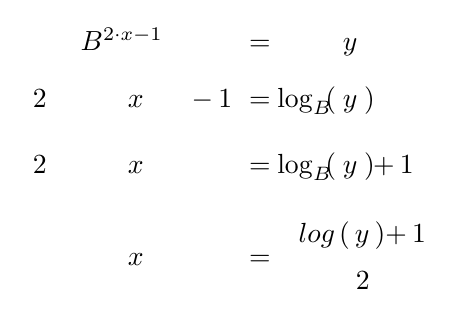
\begin{tikzpicture}[x=1em,y=-1em]
\node[anchor=base, inner sep=0pt] at (3.4,2.72) {$\pFourCell{5.04}{B^{{\scriptstyle 2\cdot{}x-1}}}$};
\node[anchor=base, inner sep=0pt] at (8.39,2.72) {$\pFourCell{1.62}{=}$};
\node[anchor=base, inner sep=0pt] at (11.65,2.72) {$\pFourCell{0.9}{y}$};
\node[anchor=base, inner sep=0pt] at (0.44,4.79) {$\pFourCell{0.88}{2}$};
\node[anchor=base, inner sep=0pt] at (3.91,4.79) {$\pFourCell{4.02}{x}$};
\node[anchor=base, inner sep=0pt] at (6.31,4.79) {$\pFourCell{0.78}{-}$};
\node[anchor=base, inner sep=0pt] at (7.14,4.79) {$\pFourCell{0.88}{1}$};
\node[anchor=base, inner sep=0pt] at (8.39,4.79) {$\pFourCell{1.62}{=}$};
\node[anchor=base, inner sep=0pt] at (10.01,4.79) {$\pFourCell{1.62}{\pFourCell{1.62}{\log_{B}}}$};
\node[anchor=base, inner sep=0pt] at (11.01,4.79) {$\pFourCell{0.38}{\left(\rule[-0.28em]{0pt}{0.8em}\right.}$};
\node[anchor=base, inner sep=0pt] at (11.65,4.79) {$\pFourCell{0.9}{y}$};
\node[anchor=base, inner sep=0pt] at (12.29,4.79) {$\pFourCell{0.38}{\left.\rule[-0.28em]{0pt}{0.8em}\right)}$};
\node[anchor=base, inner sep=0pt] at (0.44,7.19) {$\pFourCell{0.88}{2}$};
\node[anchor=base, inner sep=0pt] at (3.91,7.19) {$\pFourCell{4.02}{x}$};
\node[anchor=base, inner sep=0pt] at (8.39,7.19) {$\pFourCell{1.62}{=}$};
\node[anchor=base, inner sep=0pt] at (10.01,7.19) {$\pFourCell{1.62}{\pFourCell{1.62}{\log_{B}}}$};
\node[anchor=base, inner sep=0pt] at (11.01,7.19) {$\pFourCell{0.38}{\left(\rule[-0.28em]{0pt}{0.8em}\right.}$};
\node[anchor=base, inner sep=0pt] at (11.65,7.19) {$\pFourCell{0.9}{y}$};
\node[anchor=base, inner sep=0pt] at (12.29,7.19) {$\pFourCell{0.38}{\left.\rule[-0.28em]{0pt}{0.8em}\right)}$};
\node[anchor=base, inner sep=0pt] at (12.87,7.19) {$\pFourCell{0.78}{+}$};
\node[anchor=base, inner sep=0pt] at (13.7,7.19) {$\pFourCell{0.88}{1}$};
\node[anchor=base, inner sep=0pt] at (12.11,10.49) {$\pFourFraction{5.82em}{\makebox[5.82em][c]{\ensuremath{\pFourCell{1.62}{log}\pFourCell{0.38}{(}\pFourCell{0.9}{y}\pFourCell{0.38}{)}\pFourCell{0.78}{+}\pFourCell{0.88}{1}}}}{\makebox[5.82em][c]{\ensuremath{\pFourCell{0.88}{2}}}}$};
\node[anchor=base, inner sep=0pt] at (3.91,10.49) {$\pFourCell{4.02}{x}$};
\node[anchor=base, inner sep=0pt] at (8.39,10.49) {$\pFourCell{1.62}{=}$};
\end{tikzpicture}
\end{center}


\newpage
\section*{Spaltentreue LaTeX-Ausgabe mit Spaltengrenzen}
\vspace{6mm}
\begin{center}
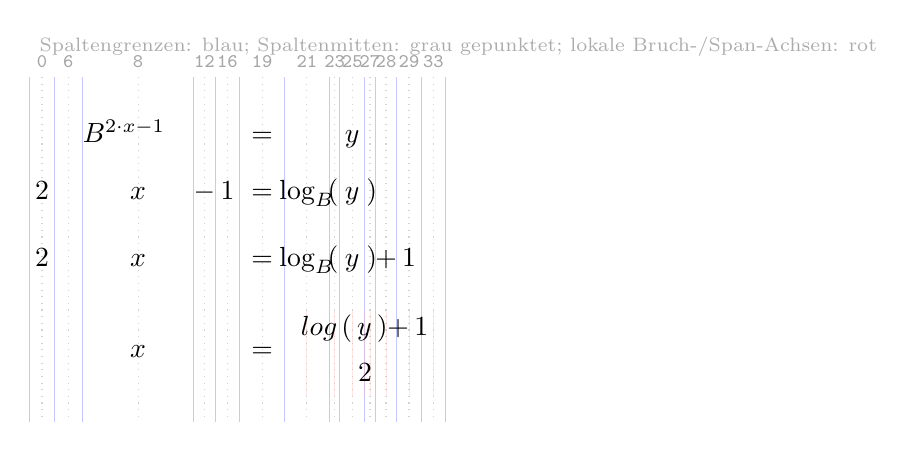
\begin{tikzpicture}[x=1em,y=-1em]
\node[font={\scriptsize}, text=gray!65, anchor=west] at (0,-0.75) {Spaltengrenzen: blau; Spaltenmitten: grau gepunktet; lokale Bruch-/Span-Achsen: rot};
\draw[blue!22, line width=0.28pt] (0,0.35) -- (0,12.82);
\draw[blue!22, line width=0.28pt] (0.88,0.35) -- (0.88,12.82);
\draw[blue!22, line width=0.28pt] (1.9,0.35) -- (1.9,12.82);
\draw[blue!22, line width=0.28pt] (5.92,0.35) -- (5.92,12.82);
\draw[blue!22, line width=0.28pt] (6.7,0.35) -- (6.7,12.82);
\draw[blue!22, line width=0.28pt] (7.58,0.35) -- (7.58,12.82);
\draw[blue!22, line width=0.28pt] (9.2,0.35) -- (9.2,12.82);
\draw[blue!22, line width=0.28pt] (10.82,0.35) -- (10.82,12.82);
\draw[blue!22, line width=0.28pt] (11.2,0.35) -- (11.2,12.82);
\draw[blue!22, line width=0.28pt] (12.1,0.35) -- (12.1,12.82);
\draw[blue!22, line width=0.28pt] (12.48,0.35) -- (12.48,12.82);
\draw[blue!22, line width=0.28pt] (13.26,0.35) -- (13.26,12.82);
\draw[blue!22, line width=0.28pt] (14.14,0.35) -- (14.14,12.82);
\draw[blue!22, line width=0.28pt] (15.02,0.35) -- (15.02,12.82);
\draw[gray!35, dotted] (0.44,0.35) -- (0.44,12.82);
\node[font={\ttfamily\scriptsize}, text=gray!70, anchor=base] at (0.44,0) {0};
\draw[gray!35, dotted] (1.39,0.35) -- (1.39,12.82);
\node[font={\ttfamily\scriptsize}, text=gray!70, anchor=base] at (1.39,0) {6};
\draw[gray!35, dotted] (3.91,0.35) -- (3.91,12.82);
\node[font={\ttfamily\scriptsize}, text=gray!70, anchor=base] at (3.91,0) {8};
\draw[gray!35, dotted] (6.31,0.35) -- (6.31,12.82);
\node[font={\ttfamily\scriptsize}, text=gray!70, anchor=base] at (6.31,0) {12};
\draw[gray!35, dotted] (7.14,0.35) -- (7.14,12.82);
\node[font={\ttfamily\scriptsize}, text=gray!70, anchor=base] at (7.14,0) {16};
\draw[gray!35, dotted] (8.39,0.35) -- (8.39,12.82);
\node[font={\ttfamily\scriptsize}, text=gray!70, anchor=base] at (8.39,0) {19};
\draw[gray!35, dotted] (10.01,0.35) -- (10.01,12.82);
\node[font={\ttfamily\scriptsize}, text=gray!70, anchor=base] at (10.01,0) {21};
\draw[gray!35, dotted] (11.01,0.35) -- (11.01,12.82);
\node[font={\ttfamily\scriptsize}, text=gray!70, anchor=base] at (11.01,0) {23};
\draw[gray!35, dotted] (11.65,0.35) -- (11.65,12.82);
\node[font={\ttfamily\scriptsize}, text=gray!70, anchor=base] at (11.65,0) {25};
\draw[gray!35, dotted] (12.29,0.35) -- (12.29,12.82);
\node[font={\ttfamily\scriptsize}, text=gray!70, anchor=base] at (12.29,0) {27};
\draw[gray!35, dotted] (12.87,0.35) -- (12.87,12.82);
\node[font={\ttfamily\scriptsize}, text=gray!70, anchor=base] at (12.87,0) {28};
\draw[gray!35, dotted] (13.7,0.35) -- (13.7,12.82);
\node[font={\ttfamily\scriptsize}, text=gray!70, anchor=base] at (13.7,0) {29};
\draw[gray!35, dotted] (14.58,0.35) -- (14.58,12.82);
\node[font={\ttfamily\scriptsize}, text=gray!70, anchor=base] at (14.58,0) {33};
\node[anchor=base, inner sep=0pt] at (3.4,2.72) {$\pFourCell{5.04}{B^{{\scriptstyle 2\cdot{}x-1}}}$};
\node[anchor=base, inner sep=0pt] at (8.39,2.72) {$\pFourCell{1.62}{=}$};
\node[anchor=base, inner sep=0pt] at (11.65,2.72) {$\pFourCell{0.9}{y}$};
\node[anchor=base, inner sep=0pt] at (0.44,4.79) {$\pFourCell{0.88}{2}$};
\node[anchor=base, inner sep=0pt] at (3.91,4.79) {$\pFourCell{4.02}{x}$};
\node[anchor=base, inner sep=0pt] at (6.31,4.79) {$\pFourCell{0.78}{-}$};
\node[anchor=base, inner sep=0pt] at (7.14,4.79) {$\pFourCell{0.88}{1}$};
\node[anchor=base, inner sep=0pt] at (8.39,4.79) {$\pFourCell{1.62}{=}$};
\node[anchor=base, inner sep=0pt] at (10.01,4.79) {$\pFourCell{1.62}{\pFourCell{1.62}{\log_{B}}}$};
\node[anchor=base, inner sep=0pt] at (11.01,4.79) {$\pFourCell{0.38}{\left(\rule[-0.28em]{0pt}{0.8em}\right.}$};
\node[anchor=base, inner sep=0pt] at (11.65,4.79) {$\pFourCell{0.9}{y}$};
\node[anchor=base, inner sep=0pt] at (12.29,4.79) {$\pFourCell{0.38}{\left.\rule[-0.28em]{0pt}{0.8em}\right)}$};
\node[anchor=base, inner sep=0pt] at (0.44,7.19) {$\pFourCell{0.88}{2}$};
\node[anchor=base, inner sep=0pt] at (3.91,7.19) {$\pFourCell{4.02}{x}$};
\node[anchor=base, inner sep=0pt] at (8.39,7.19) {$\pFourCell{1.62}{=}$};
\node[anchor=base, inner sep=0pt] at (10.01,7.19) {$\pFourCell{1.62}{\pFourCell{1.62}{\log_{B}}}$};
\node[anchor=base, inner sep=0pt] at (11.01,7.19) {$\pFourCell{0.38}{\left(\rule[-0.28em]{0pt}{0.8em}\right.}$};
\node[anchor=base, inner sep=0pt] at (11.65,7.19) {$\pFourCell{0.9}{y}$};
\node[anchor=base, inner sep=0pt] at (12.29,7.19) {$\pFourCell{0.38}{\left.\rule[-0.28em]{0pt}{0.8em}\right)}$};
\node[anchor=base, inner sep=0pt] at (12.87,7.19) {$\pFourCell{0.78}{+}$};
\node[anchor=base, inner sep=0pt] at (13.7,7.19) {$\pFourCell{0.88}{1}$};
\draw[red!30, opacity=0.32, line width=0.35pt] (10.01,8.79) -- (10.01,11.92);
\draw[red!30, opacity=0.32, line width=0.35pt] (10.82,8.79) -- (10.82,11.92);
\draw[red!30, opacity=0.32, line width=0.35pt] (11.01,8.79) -- (11.01,11.92);
\draw[red!30, opacity=0.32, line width=0.35pt] (11.2,8.79) -- (11.2,11.92);
\draw[red!30, opacity=0.32, line width=0.35pt] (11.65,8.79) -- (11.65,11.92);
\draw[red!30, opacity=0.32, line width=0.35pt] (12.1,8.79) -- (12.1,11.92);
\draw[red!30, opacity=0.32, line width=0.35pt] (12.29,8.79) -- (12.29,11.92);
\draw[red!30, opacity=0.32, line width=0.35pt] (12.87,8.79) -- (12.87,11.92);
\draw[red!30, opacity=0.32, line width=0.35pt] (13.7,8.79) -- (13.7,11.92);
\draw[red!30, opacity=0.32, line width=0.35pt] (14.14,8.79) -- (14.14,11.92);
\draw[red!30, opacity=0.32, line width=0.35pt] (14.14,8.79) -- (14.14,11.92);
\draw[red!30, opacity=0.32, line width=0.35pt] (14.14,8.79) -- (14.14,11.92);
\draw[red!30, opacity=0.32, line width=0.35pt] (14.58,8.79) -- (14.58,11.92);
\node[anchor=base, inner sep=0pt] at (12.11,10.49) {$\pFourFraction{5.82em}{\makebox[5.82em][c]{\ensuremath{\pFourCell{1.62}{log}\pFourCell{0.38}{(}\pFourCell{0.9}{y}\pFourCell{0.38}{)}\pFourCell{0.78}{+}\pFourCell{0.88}{1}}}}{\makebox[5.82em][c]{\ensuremath{\pFourCell{0.88}{2}}}}$};
\node[anchor=base, inner sep=0pt] at (3.91,10.49) {$\pFourCell{4.02}{x}$};
\node[anchor=base, inner sep=0pt] at (8.39,10.49) {$\pFourCell{1.62}{=}$};
\end{tikzpicture}
\end{center}
\end{document}
